\documentclass[18pt]{article}
\usepackage[utf8]{inputenc}
\usepackage[T1]{fontenc}
\usepackage{ragged2e}
\usepackage{caladea}
\usepackage{graphicx}
\usepackage{longtable}
\usepackage{wrapfig}
\usepackage{rotating}
\usepackage{epigraph}
\usepackage[normalem]{ulem}
\usepackage{hyperref}
\usepackage{amsmath}
\usepackage{amssymb}
\usepackage{capt-of}
\usepackage{hyperref}
\usepackage{fancyhdr}

\title{
 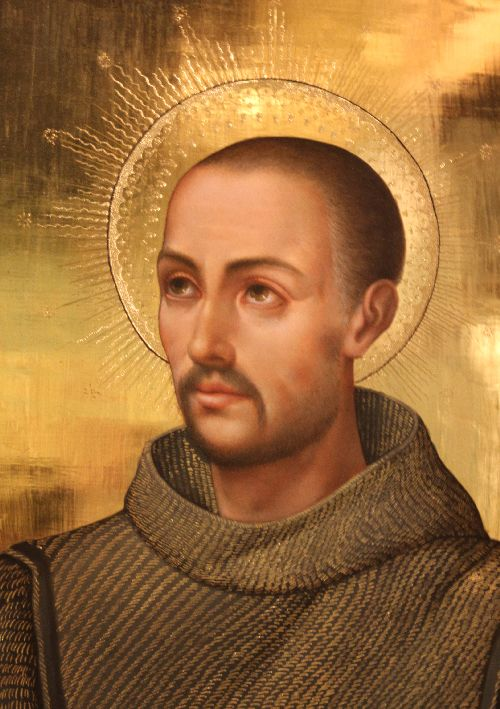
\includegraphics[scale=.6, trim={10cm, 0, 10cm, 0}]{./assets/imagem.jpg}
  \par
 NOVENA SÃO JOÃO DE DEUS}
\date{Data Litúrgica: 08/03 }

% Comando para fazer "Sumário" não aparecer no Sumário.
\renewcommand{\contentsname}{Sumário}
\begin{document}
\maketitle

\thispagestyle{empty} %zera a primeira página

\pagestyle{fancy}
\fancyhf{} % clear existing header/footer entries
\fancyfoot[LO, CE]{
 
\includegraphics[scale=0.2]{./assets/cross.png} São João de Deus, Rogai por nós!
}
% Place Page X of Y on the right-hand
% side of the footer
\fancyfoot[R]{\thepage}

\newpage

\tableofcontents

\centering
\vfill
Visite-nos no Telegram: \url{https://t.me/CotidieNovena}
\newpage

\newpage


%%%%%%%%%%%%%%%%%%%%%%%%%%%%%%%%%%%%% Orações %%%%%%%%%%%%%%%%%%%%%%%%%%%%%%%%%%%%%%%%%%%

\begin{justify}

 \begin{center}
  \section{História}\label{sec:História} % (fold)
 \end{center}

No então, claro, ainda não tinha chegado o momento certo. Ao chegar a Oropesa, na Espanha, João morou com uma família de pastores até aos 27 anos; depois, alistou-se no Exército e combateu pelo menos duas batalhas importantes em Pavia e em Viena, invadidas pelos Turcos. Mais tarde, enquanto tinha dinheiro, viajou por todo o continente europeu até chegar à África. A seguir, retornou à Espanha e se instalou em Granada, onde abriu uma livraria. Entre todos os empregos que teve até então, o de ser livreiro foi o que mais gostou: apaixonou-se logo pelos livros, que os considerou também como uma ajuda para a oração e a fé, sobretudo aqueles com imagens sagradas.

Certo dia, em Granada, João ouviu um sermão do místico João de Ávila que o iluminou. Então, começou a sair pelas ruas pedindo esmolas para os pobres, utilizando uma fórmula especial em três palavras: "Façam o bem, irmãos", exortando os outros a fazerem o bem ao próximo, mas também a si mesmos. Ao mesmo tempo, começou, igualmente, a praticar formas tão clamorosas de penitência, que o levaram a ser preso e a acabar em um manicômio. Ali, João descobriu os últimos entre os doentes, trancados por suas famílias para se esconder e se livrar deles. Além do mais, tocou com as mãos os métodos com os quais eram curados, quase como verdadeiras torturas. Assim, entendeu que deveria fazer algo para aqueles irmãos mais infelizes, porque Deus queria.

Quando terminou a sua experiência no manicômio, João foi ter com o Bispo, diante do qual se comprometeu em viver pelos que sofriam e a acolher os que quisessem fazer a mesma coisa. A Providência deu-lhe dois confrades: todos os três usaram um pobre saio, com uma cruz vermelha, fundando assim, em 1540, o primeiro núcleo da Congregação dos Irmãos da Misericórdia. Mas, João queria ir mais além. Apesar de não ter noções de medicina, estava ciente de que devia tratar dos doentes de modo novo, ou seja, ouvindo-os e satisfazendo as suas necessidades de diversas maneiras. Desta forma, conseguiu fundar um primeiro hospital, segundo estes ditames, em Granada e, depois, em Toledo, dedicando-se, ao mesmo tempo, aos órfãos, prostitutas e desempregados.

João faleceu aos 55 anos, em 1550, enquanto rezava de joelhos e apertava ao peito um crucifixo. Ele não deixou nenhuma Regra escrita, mas a sua obra de caridade já estava bem encaminhada e seus coirmãos continuavam inspirados por ele. Quarenta e cinco anos mais tarde, seus ensinamentos foram codificados na Regra concernente à nova Ordem hospitaleira de São João de Deus, também chamada, precisamente como o seu nome - "Fatebenefratelli".
São João de Deus foi canonizado em 1609 e proclamado Padroeiro dos enfermos e dos hospitais.

\begin{center}
 \subsection*{Créditos:}
 \href{https://www.vaticannews.va/pt/santo-do-dia/03/08/s--joao-de-deus--fundador-da-ordem-hospitaleira--padroeiro-dos-d.html}{Vatican News}
\end{center}


\end{justify}
%%%%%%%%%%%%%%%%%%%%%%%%%%%%%%%%%%%%% Orações %%%%%%%%%%%%%%%%%%%%%%%%%%%%%%%%%%%%%%%%%%%
\begin{justify}

\newpage
\begin{center}
 \section{Orações}\label{sec:Orações} % (fold)
\textit{Em nome do Pai, e do Filho, e do Espírito Santo. Amém.}
\end{center}

\begin{center}
\subsection{Oração Inicial}\label{sec:Oração_Inicial} % (fold)
\end{center}

São João de Deus, patrono celestial dos enfermos, venho a você em oração para buscar sua ajuda em minha atual enfermidade. Através do amor que Jesus teve por você ao escolhê-lo para a sublime vocação de servir os doentes, e pela ternura com que a Bem-Aventurada Virgem Maria colocou sobre sua cabeça uma coroa de espinhos como símbolo dos sofrimentos que você enfrentaria no serviço aos enfermos para alcançar sua coroa de glória, peço que interceda por mim junto a Jesus e Maria, para que Eles possam me conceder uma cura, se isso estiver de acordo com a Vontade de Deus. Como você suportou pacientemente os sofrimentos de sua própria doença! Ensine-me a carregar com alegre resignação a cruz que Deus me deu. Que eu nunca me queixe ou perca a coragem. Ajude-me a entender que o sofrimento é um meio muito importante de santificar minha alma, de expiar meus muitos pecados e de colher uma abundante colheita de méritos para o Céu. Confio em seu grande amor pelos enfermos e no poder de sua intercessão para ajudá-los.

Ajude-me, bom Santo, e implore ao Deus cujo nome você carrega que me toque como Ele tocou os enfermos enquanto estava na terra, para que, através de Seu poder onipotente, a saúde possa retornar ao meu corpo. E assim como você encontrou força em seus próprios sofrimentos na cruz, que eu possa ser capaz de dizer o que você disse a Jesus Crucificado: “Senhor, Teus espinhos são minhas rosas e Teus sofrimentos meu paraíso.” Bom São João, amante dos que sofrem e especial Patrono dos Enfermos, coloco confiantemente diante de você meu pedido sincero.

\textit{\textbf{(Mencione seu pedido aqui…)}}

Peço que recomende meu pedido a Maria, Mãe das Dores e Saúde dos Enfermos, para que tanto Maria quanto você possam apresentá-lo a Jesus, o Divino Médico. São João de Deus, patrono dos Enfermos e amado de Jesus e Maria, ore por mim e obtenha meu pedido. (Três vezes.)



\begin{center}
 \subsection{Oração Final}\label{sec:Oração_Final} % (fold)
\end{center}


\begin{center}
\textbf{Pai Nosso, Ave Maria, Glória ao Pai.}

\vfill
\section*{São João de Deus, rogai por nós!}

\vfill
\subsection*{Créditos:}
\href{https://novenaprayer.com/st-john-of-god-novena/}{Novena Prayer}

\end{center}


\end{justify}

\end{document}
